\chapter{HIV/AIDS Awareness}

This section was originally prepared for the Biology Sourcebook of the Mzumbe Book Project by Mr. M. Sawaya of the Inspectorate, Ministry of Education and Culture, Dar es Salaam.

\section{Introduction}

The purpose of this material is to provide a guide or basis for the school AIDS education
program. On the grounds that the future of our nation and progress is based on the on going
generation - the student. Hence the aim is to promote behaviour which will reduce
transmission of HIV among young people.

The main mode of HIV transmission is through unprotected sexual intercourse. Open talk on
sex is difficult in our society, thus making discussions on AIDS education a sensitive issue
which has to touch on personal, religious cultural and moral perspectives. Initial and
continuous communication on all aspects of education is expected and requires time,
cooperation and participation of many people from the school, the home and the community.
Teachers who are going to do much of the education have to change their attitudes towards
students. They have to treat students as individuals and with respect. They have to make
students become comfortable and confident to talk about sexuality and related issues freely
with them. It is advised that interpersonal relationship between teacher and student is
fostered as it is the basis for preventive education and counselling.

The AIDS education provided in this material considers it as part of integrated health
education program. AIDS or HIV infection is not treated as a set of isolated disease, but
understanding it as disease that needs action to prevent or limit its development through
learning and practising positive health behaviour, skills and attitudes. Likewise importance, is
linked to Family life Education were self-esteem, respect for self and others, decision making
nurturing relationships. That will help students to understand the immediate and long term
benefits of abstaining from sexual activity.

\begin{center}
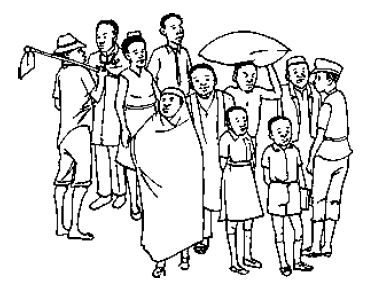
\includegraphics[width=0.6\textwidth]{./img/source/aids-1.jpg}
\end{center}

\section{AIDS - Current Information}

This brief overview provides teachers with a general understanding of AIDS. It should be
supplemented as needed with other texts on the subject. Knowledge about the disease and
its effects on individuals is constantly being updated.

\noindent \textbf{Teachers should periodically review and update this information to assure that is
accurate.}

\section{Description and Cause of AIDS}

\begin{itemize}
\item Acquired Immune Deficiency Syndrome (AIDS) is a disease caused by a virus that
attacks the body's immune system, making infected people vulnerable to opportunistic
infections, cancer, and neurological disorders.
\item The AIDS virus (called Human Immunodeficiency Virus-HIV) primarily attacks certain
white blood cells (called T-Lymphocytes or T-4 helper cells) that are part of the body's
internal defense against disease. The virus may also attack the central nervous system.
\item An infected person's immune system responds by developing antibodies to fight off the
invading virus. It is these antibodies to HIV, and not the virus itself, that can be identified
by a blood test before a person has any signs of illness. However, the body's ability to
produce disease-fighting antibodies eventually becomes limited in HIV-infected persons as
the virus reproduces and multiplies, killing the critical T-4 cells it has infected.
\end{itemize}

\section{Clinical Manifestations}

\begin{itemize}
\item HIV infection may lead to disease which can take many forms. It ranges from the
complete absence of symptoms to mild illness, to debilitating neurological disorders, and
to fatal disease.
\item The condition called AIDS represents a syndrome of late-stage diseases in which the
immune system is unable to fight off other viruses, bacteria, protozoa, and fungi, resulting
in infections and diseases that eventually cause the death o
\item The condition called AIDS Related Complex (ARC) refers to individuals who have a
suppressed immune system and symptoms of AIDS but no specific opportunistic
infections. For an unknown percentage of individuals, ARC is a precursor to AIDS.
\item The onset of symptoms associated with either ARC or AIDS may take from six months to
five or more years to appear after the virus has entered the body. At this time most
individuals exposed to HIV do not develop either ARC or AIDS, although they are carriers
of the virus and are capable of infecting others.
\item Symptoms related to ARC include:
	\begin{itemize}
	\item loss of appetite
	\item weight loss
	\item fever
	\item night sweats
	\item skin, rashes
	\item diarrhoea
	\item tiredness
	\item lack of resistance to infection
	\item swollen lymph glands
	\end{itemize}
	The symptoms are likely to be milder than those found in person with AIDS and generally are
present in a cyclic fashion with illness followed by periods of wellness.
\item The symptoms that individuals with AIDS develop are related to the opportunistic
diseases that have taken advantage of the compromised immune response due to HIV
infection. These symptoms are usually persistent and difficult to treat, and they
progressively debilitate the person to the point of death. They may include:
	\begin{itemize}
	\item extreme tiredness, sometimes combined with headaches, dizziness, or
lightheadedness
	\item continued fever or night sweats
	\item weight loss of more than 10 pounds that is not due to dieting or increased physical
activity
	\item swollen glands in the neck, armpits, or groin
	\item purple or discoloured growths on the skin or the mucous membranes (inside the
mouth, anus, or nasal passages)
	\item heavy, continual dry cough that is not from smoking or that has lasted too long to be a
cold or flu
	\item continuing bouts of diarrhoea
	\item thrush (a thick whitish coating on the tongue or in the throat), which may be
accompanied by sore throat
	\item unexplained bleeding from any body opening or from growths on the skin or mucous
membranes
	\item bruising more easily than usual
	\item progressive shortness of breath
	\item confusion, lethargy, forgetfulness, lack of coordination, general mental deterioration.
	\end{itemize}
\item Specific diseases that generally don't affect healthy adults are linked with HIV infection.
\item The incubation period before any symptoms of HIV disease appear varies significantly
from person to person. Many infected people develop symptoms within two years of
exposure. Others, infected up to seven years ago, have not yet shown any signs of illness.
Since AIDS is a new disease, only recognized in 1981, the maximum incubation period
has not yet been identified. Extensive research is in progress to identify potential internal
or external co-factors that may cause some infected people to become fatally ill, while
others have milder symptoms or remain symptom-free.
\end{itemize}

\section{Transmission}

Unlike flu or measles, HIV is not transmitted through the air; it must get into the bloodstream
to cause infection. For this reason, HIV-infected people do not pose a risk to others through
any form of casual contact. There is no evidence that AIDS is transmitted through coughing,
sneezing, food preparation, drinking fountains, toilet seats, being around an infected person
on daily basis, or donating blood.

HIV is carried in blood, semen, vaginal secretions, and other body fluids including tears and
saliva of an infected person. It is transmitted from one person to another by three routes: 
\begin{enumerate}
\item through sexual intercourse (physical sexual contact between individuals that involves the
genitalia of at least one person-includes vaginal intercourse, oral intercourse, and anal
intercourse),
\item through parenteral exposure to infected blood, and
\item from infected women to
their infants during the perinatal period.
\end{enumerate}

Sexual transmission of the AIDS virus occurs during intercourse. It is thought that it happens
through abrasions or tiny, unfelt tears that may occur in delicate tissues. Such tissue breaks
can allow infected semen, blood, or vaginal fluid to enter the bloodstream of a sex partner.
Anal intercourse is most risky, since tissue tearing and bleeding are likely to occur.
Transmission through parenteral exposure to infected blood occurs in persons sharing
contaminated needles, syringes, and works during intravenous (IV) drug use. Small, even
invisible, particles of infected blood can remain in the drug paraphernalia and can be injected
into the bloodstream of the next user.

The risk of AIDS transmission through blood transfusions has been almost eliminated since
all blood banks began testing donated blood for antibodies to HIV in 1985. There may be
some risk to receiving blood if it was too early for the virus to show up when donor blood was
tested. Blood-donor testing has been so effective it has reduced the risk of AIDS from blood
transfusion to one in a million. There is no risk of AIDS from donating blood; blood collection
centers use new transfusion equipment for each donor.

All infected people, whether or not they have any symptoms, are presumed capable of
transmitting the virus to others through blood-to-blood or semen-to-blood exchange, or
through vaginal secretions-to-blood exchange.

An individual can be infected with the virus that causes AIDS without having symptoms of
AIDS or appearing ill. Infected individuals without symptoms can transmit the infection to
others. Once infected, a person is presumed infected for life, but actual symptoms may not
develop for many years. A single exposure to the AIDS virus may result in infection.

\subsection{How the virus is NOT known to be spread}

\begin{itemize}
\item There is no evidence that the virus is spread through casual social contact (shaking
hands, social kissing, coughing, sneezing; sharing swimming pools, bed linens, eating
utensils, office equipment; being next to or served by an infected person in ordinary social
contact). There is no reason to avoid an infected person in ordinary social contact.
\item It is not spread by the process of giving blood; new transfusion equipment is used for
each donor.
\item HIV is not transmitted by insects.
\item It is not spread by sexual intercourse between individuals who have maintained a sexual
relationship exclusively with each other, assuming that they have not been infected
through contaminated blood, blood factors, IV drug use, or a previous sexual partner.
\end{itemize}

\subsection{Major Risk Factors}

Persons at increased risk for being infected with the AIDS virus include:

\begin{itemize}
\item homosexual and bisexual men
\item sex partners of IV drug abusers
\item male or female prostitutes and their sex partners
\item sex partners of infected persons
\item all persons with haemophilia who received blood-clotting factor and transfusions prior to
1985
\item Children born to infected mothers.
\end{itemize}

\section{Prevention}

There is no vaccine against AIDS or any treatment so far that can reverse AIDS damage to
the immune system. People must learn how to protect themselves and their loved ones from
this infection. It is essential that students gain knowledge and skills to protect themselves
before they reach an age at which they might experiment with sex or illegal drugs. Following
are some basic elements of AIDS information related to prevention.

\subsection{How to Prevent Infection}

\begin{itemize}
\item Infection through sexual contact can be avoided by practicing abstinence or having a
mutually monogamous marriage/relationship with no known risk factors in either partner.
Young people can stay safe from AIDS by not having sex. They need to know it is all right
to \textbf{say NO}. In addition to the risk of AIDS, there are other health reasons to postpone sex,
including the risk of gonorrhea, syphilis, and herpes, and unplanned pregnancies.
\item Do not use IV drugs; do not share needle or works. Young people can stay safe from
AIDS by not using IV drugs. They need to know it is all right to say NO not only to IV drugs
but to alcohol and drugs of any kind, as these impair judgment. In addition to the risk of
AIDS, there are many other health reasons for abstaining from illegal drug use.
\item If already sexually active:
	\begin{itemize}
	\item Until you ask a lot of questions about his or her past sexual experience and drug use,
don't have sex with anyone.
	\item The more people you have sex with, the greater the chance you may get infected, so
don't have sex with multiple partners.
	\item With infected persons, using a condom during sex may help keep the virus from
getting into your body. A condom is a thin rubber covering that is slipped over the penis
before any sexual contact. (See \nameref{sec:condoms}.)
	\item The chance of blood or semen entering your bloodstream is very high during anal sex,
since it can cause tearing of delicate tissues, so avoid anal sex.
	\item Drugs and alcohol can lead you to do things you wouldn't do drug-free, so don't drink
alcohol or use drugs of any kind.
	\end{itemize}
\end{itemize}

\subsection{If There is Suspicion of Infection}

\begin{itemize}
\item Abstain from sexual intercourse.
\item Seek counseling and AIDS virus antibody testing to be sure of infection status. Be aware
that weeks to months may elapse from the time of infection to the time that antibodies to
the AIDS virus appear in the blood. During this time persons may be infectious but the test
may be negative.
\item Obtain counseling and testing if pregnancy is being considered.
\end{itemize}

\subsection{Information which will emphasize the seriousness of the problem, yet reduce
inappropriate fear}

\begin{itemize}
\item AIDS is a national emergency requiring attention from all citizens.
\item If people change their behaviours, the spread of the AIDS virus can be reduced.
\item Blood for transfusion in Tanzania is screened for antibodies to the HIV and is now
essentially safe, but some risks cannot be eliminated.
\item Everyone who engages in high-risk behaviour is at risk for AIDS, regardless of age, race,
or socioeconomic status.
\end{itemize}

\section{Research and Treatment}

Researchers in the Tanzania and other countries are working diligently to develop a vaccine
to protect people from HIV. Vaccine development is made more difficult because the virus can
alter its form in the human body. These is no cure for AIDS at this time, nor is there any
treatment that can restore the function of the immune system. A number of antiviral drugs
including AZT (Azidothymidine) are being tested on patients. While AZT has shown some
promise in curbing the ability of the virus to reproduce itself inside human cells, the drug is
highly toxic and has serious side effects. Some drugs used in cancer control, such as
Interferon, are also being tried with AIDS patients.

\section{Societal Issues}

When a disease epidemic threatens society, the needs of all people must be considered:
those already infected with the disease, those threatened by the disease, and those who will
provide support for others.

In the past, once treatment or medical prevention for an epidemic infection was easily
available, society sought to protect itself by providing information to as many people as
possible through school-based courses and educational campaigns and, in some cases, by
requiring mass strategies such as immunization (polio) or premarital blood tests (syphilis). As
the number of AIDS cases mounts, this epidemic will have a significant and long-term impact
on interpersonal and family relationships, medical care delivery, public policies, and health care resources. Because there is no available treatment, tremendous fears exist. Education
must be used to curb those fears that can lead to discriminatory behaviour against people
with AIDS. The rights of people with AIDS must be weighed and protected within the
framework of disease prevention and with relation to the rights of those not infected.

\section{Condoms} 
\label{sec:condoms}

A condom is a thin sheath that is placed over the erect penis to retain semen upon
ejaculation. A condom is a safe and effective device in the prevention of pregnancy and
somewhat effective in the prevention of sexually transmitted diseases, such as gonorrhoea,
syphilis, and HIV. When properly used, a condom is theoretically 90 percent effective.
However, it should be clear that, the use of condom is not an ABSOLUTE DEFENSE
AGAINST HIV INFECTION. YET, YOU WILL BE RESPONSIBLE TO USE SKILL STUDIED
TO PREVENT YOURSELF FROM HIV INFECTION.

NOT HAVING SEX IS ONE SURE WAY TO AVOID HIV INFECTION.

\subsection{How to Use the Condom}

Buy condoms that are stored out of the sun and not yet expired. MAKE SURE that the packet
with the condom is intact. Do not use brittle, damaged condoms. Keep condoms in a cool
place, away from the body's heat.

\begin{enumerate}
\item Wait for the penis to be fully erect before putting on the condom.
\item Take the condom out of the packet carefully so that it does not get torn by finger nails.
\item Pinch the end of the condom with the thumb and finger of one hand (do not let nails tear
it!) The purpose is to remove air from the tip. Place the condom on tip of the penis
\item With the other hand-roll the condom all the way down to the base of the penis.
\item Now its' ready. Only use water-based lubricants. Lubricants containing oil such as
grease, vaseline will damage condoms.
\item After ejaculating, take the penis out of the vagina before it goes soft, carefully holding
the condom onto the penis so that no sperms spills. Direct the penis downwards and
remove the condom gradually.
\item Dispose the condom in the latrine or in a way that children cannot play with it. Do not
use condoms more than once.
\end{enumerate}

